\section{Appendix}

\subsection{Simulated broadband and single Fano cavity resonance transmission spectra}

\begin{figure}[h!]
    \centering
    \begin{subfigure}[b]{0.49\textwidth}
        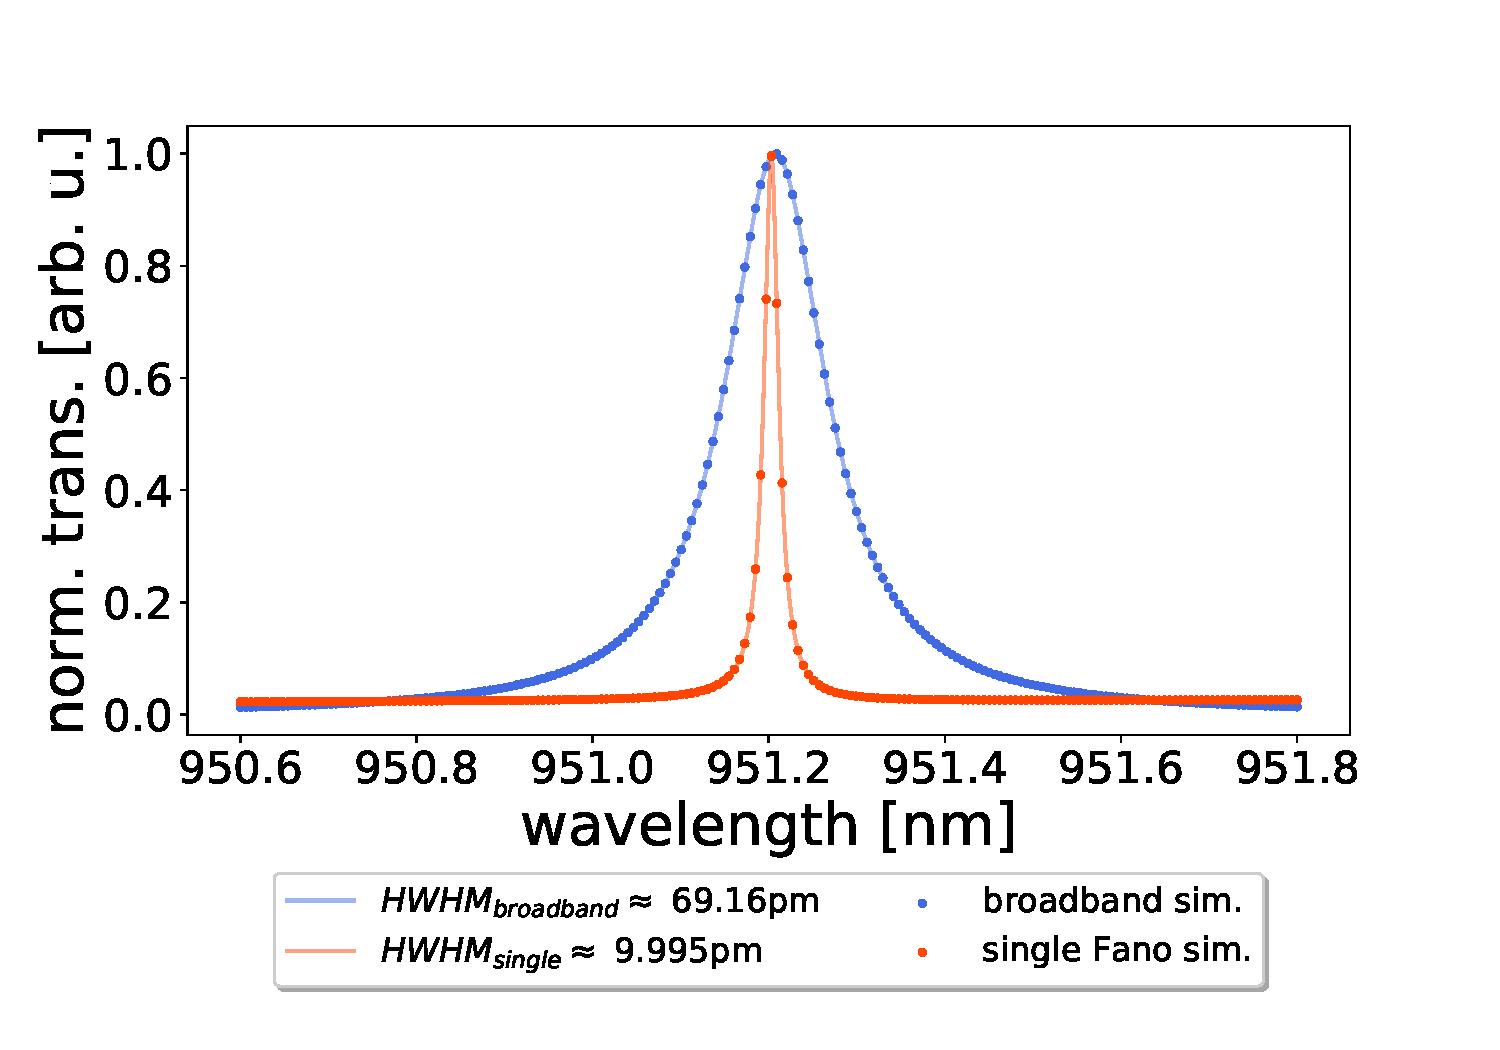
\includegraphics[width=\textwidth]{figures/sim_single_vs_broadband_10um.pdf}
        \caption{}
        \label{fig:single_vs_broadband_simulation_10um}
    \end{subfigure}
    \begin{subfigure}[b]{0.49\textwidth}
        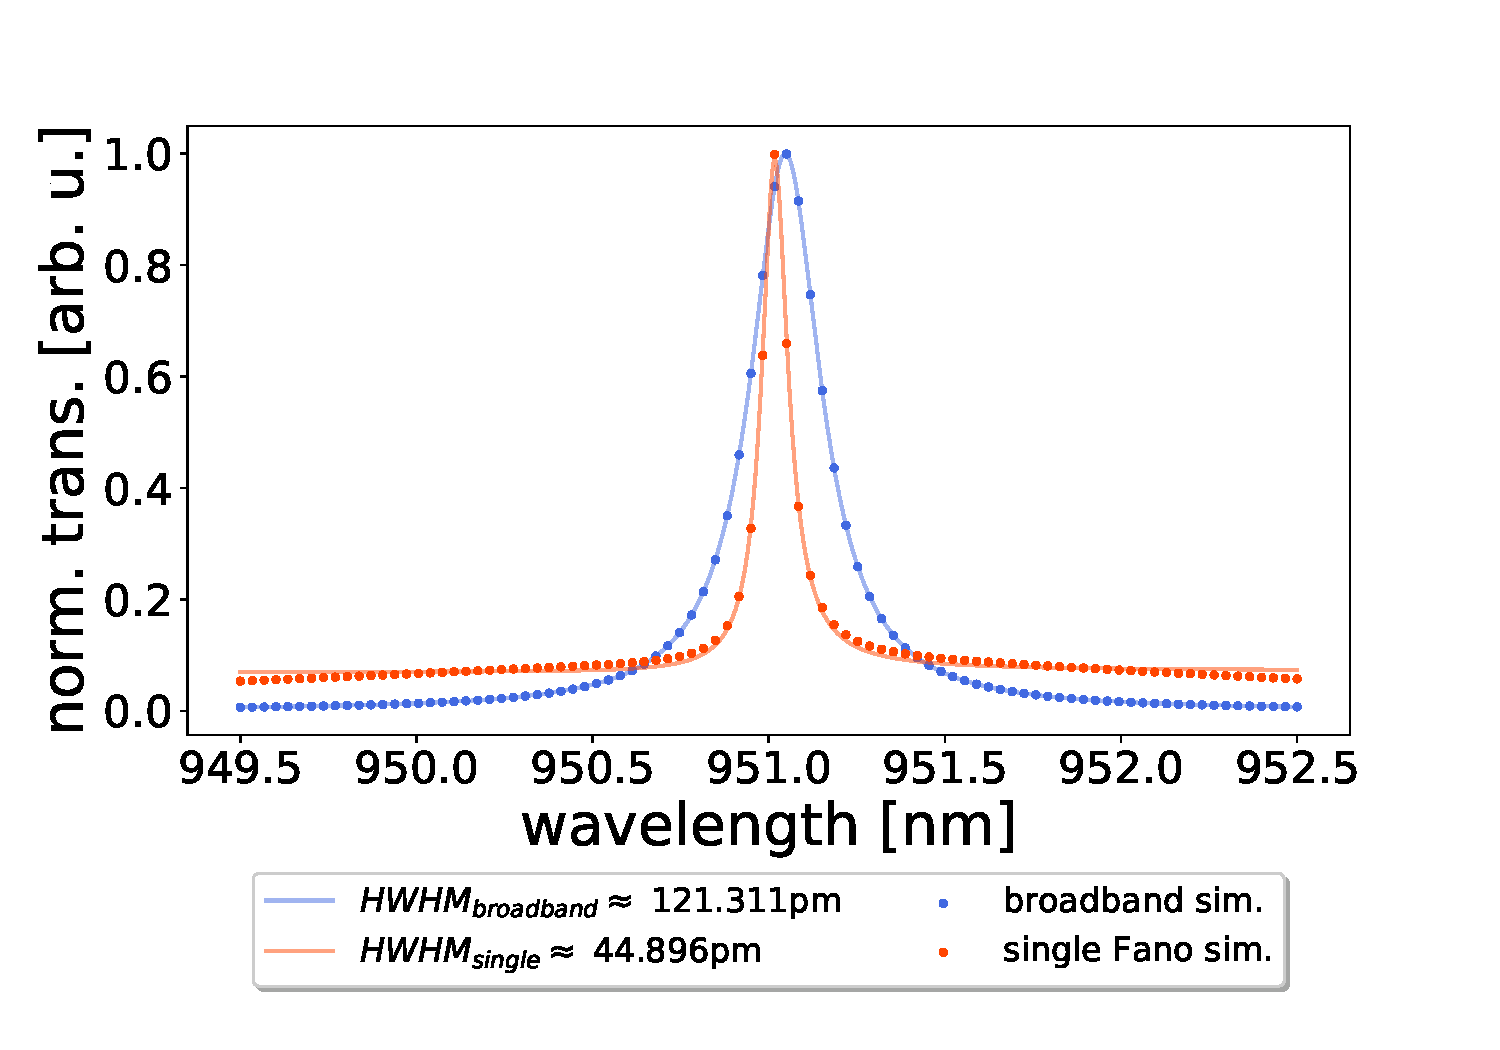
\includegraphics[width=\textwidth]{figures/sim_single_vs_broadband_30um.pdf}
        \caption{}
        \label{fig:single_vs_broadband_simulation_30um}
    \end{subfigure}
\end{figure}

\begin{figure}[h!]
    \centering
    \begin{subfigure}[b]{0.49\textwidth}
        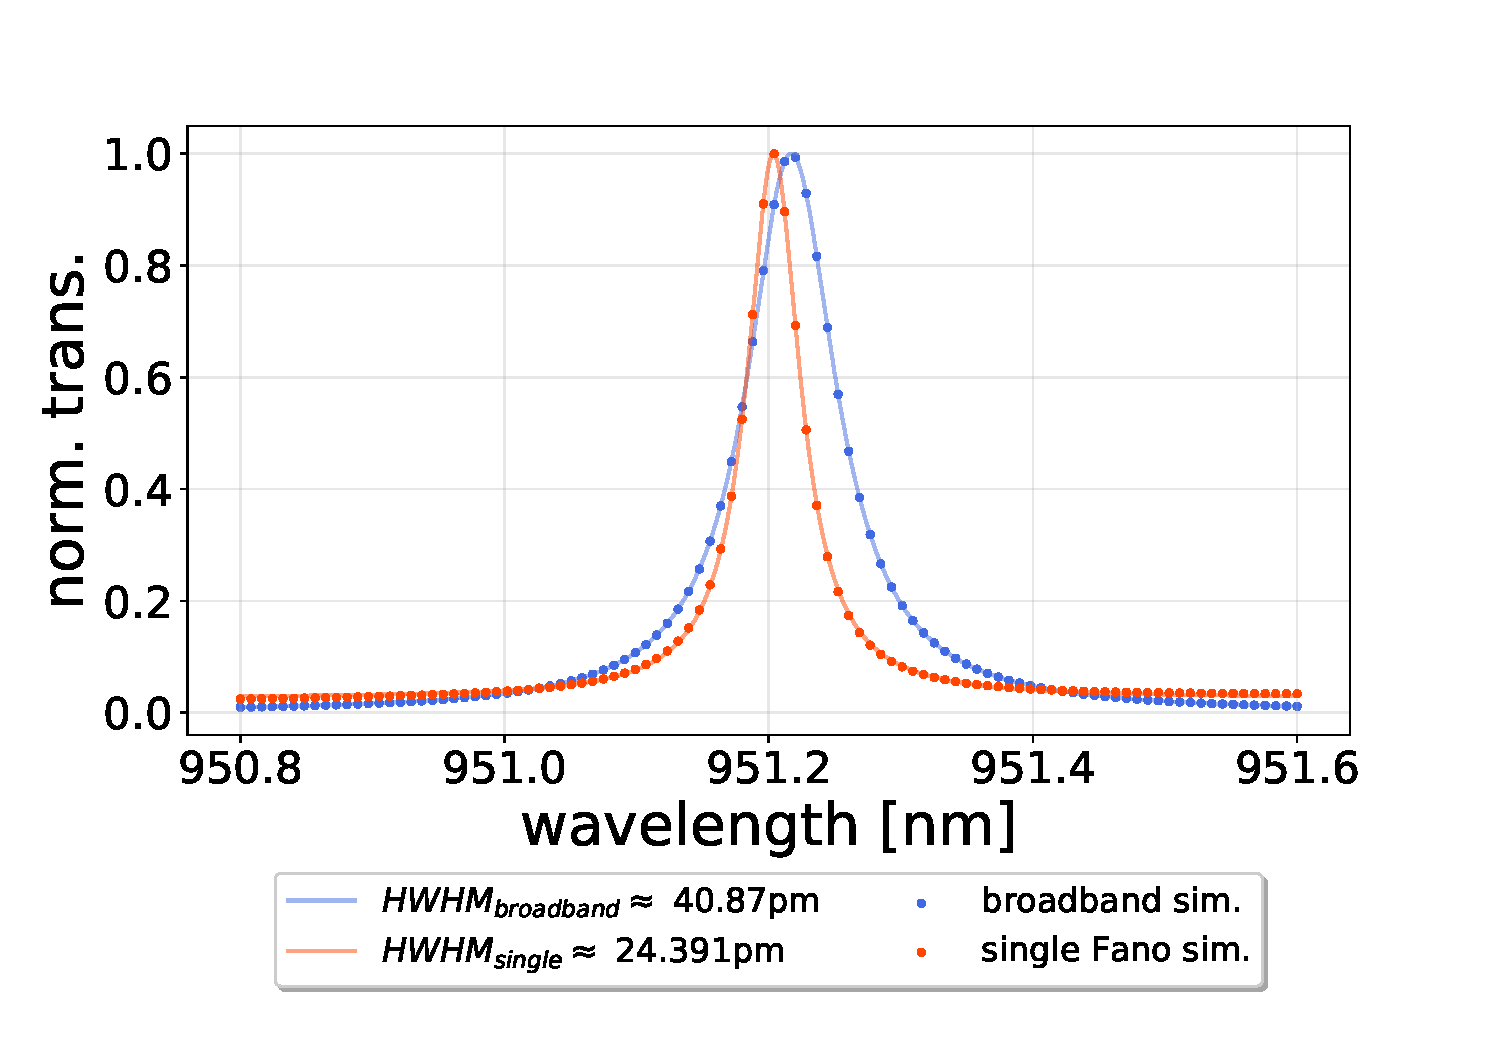
\includegraphics[width=\textwidth]{figures/sim_single_vs_broadband_90um.pdf}
        \caption{}
        \label{fig:single_vs_broadband_simulation_90um}
    \end{subfigure}
    \begin{subfigure}[b]{0.49\textwidth}
        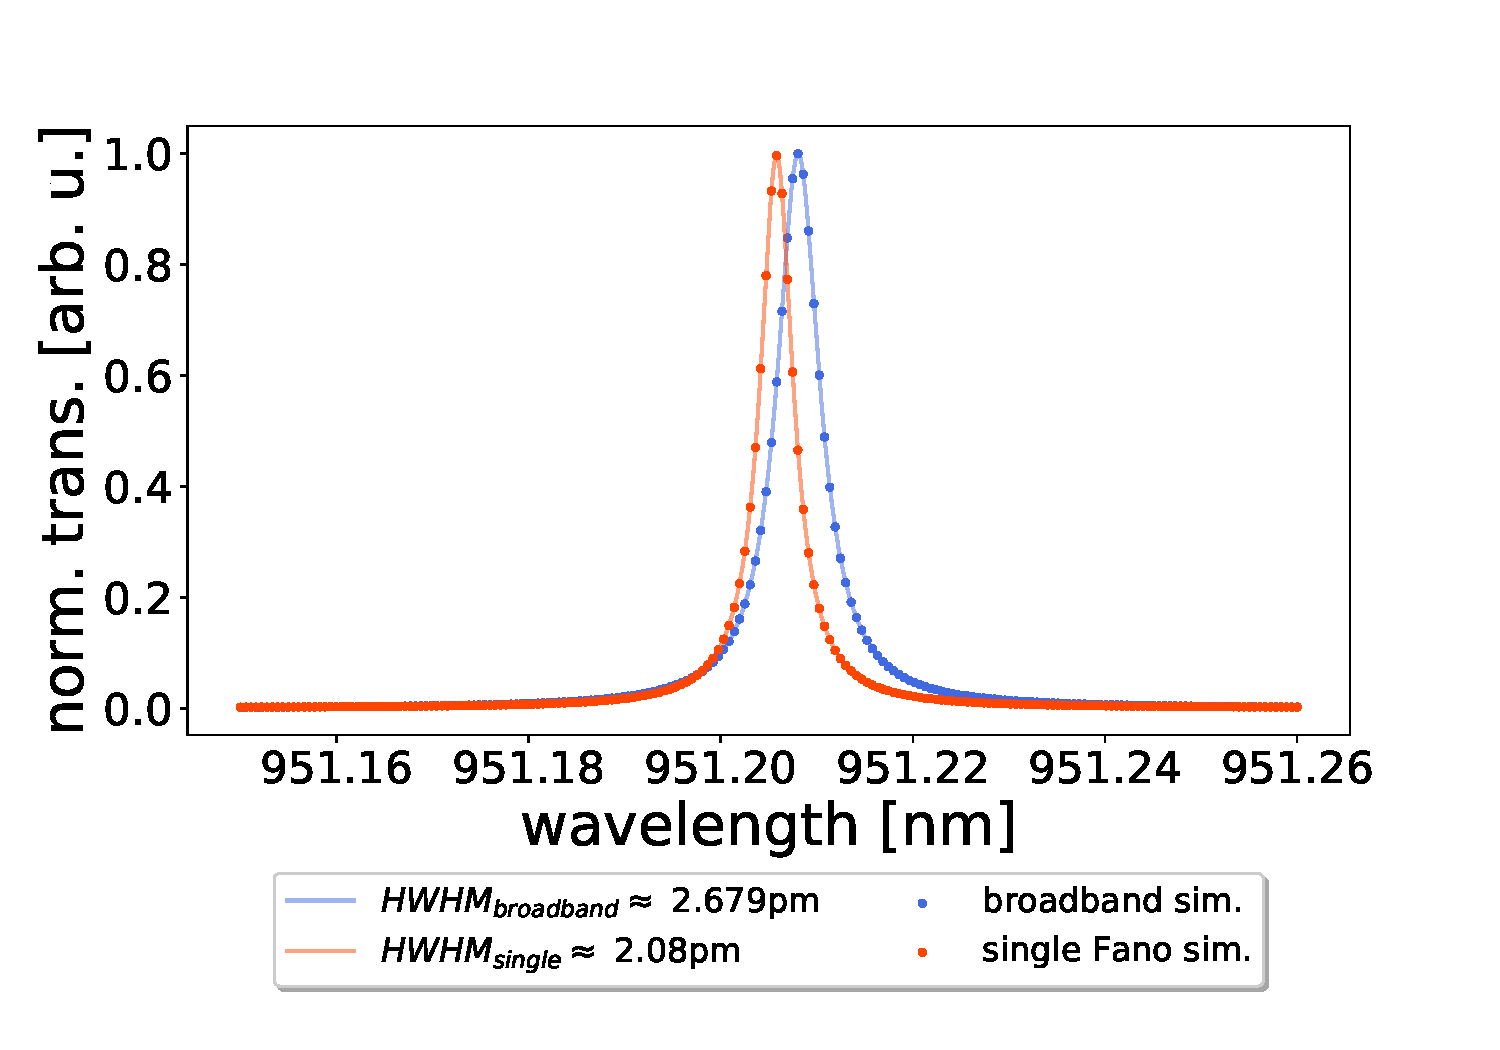
\includegraphics[width=\textwidth]{figures/sim_single_vs_broadband_270um.pdf}
        \caption{}
        \label{fig:single_vs_broadband_simulation_270um}
    \end{subfigure}
\end{figure}

\begin{figure}[h!]
    \centering
    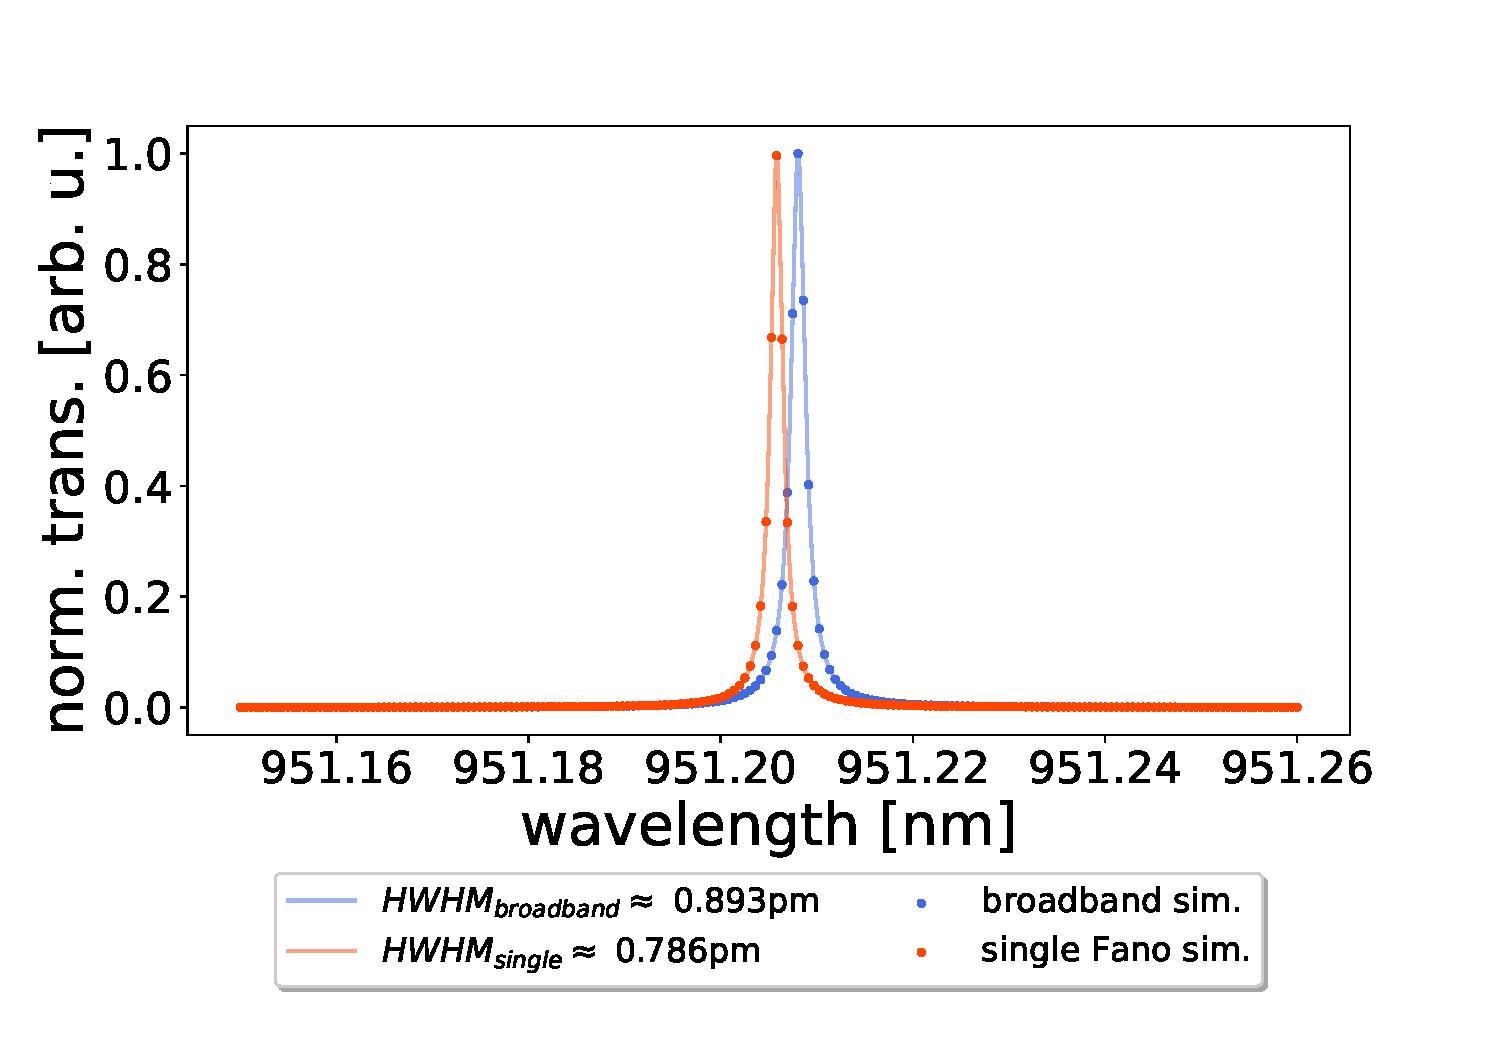
\includegraphics[width=0.49\textwidth]{figures/sim_single_vs_broadband_810um.pdf}
    \caption{}
    \label{fig:single_vs_broadband_simulation_810um}
\end{figure}

\clearpage
\subsection{Simulated single and double Fano cavity resonance transmission spectra}

\begin{figure}[h!]
    \centering
    \begin{subfigure}[b]{0.49\textwidth}
        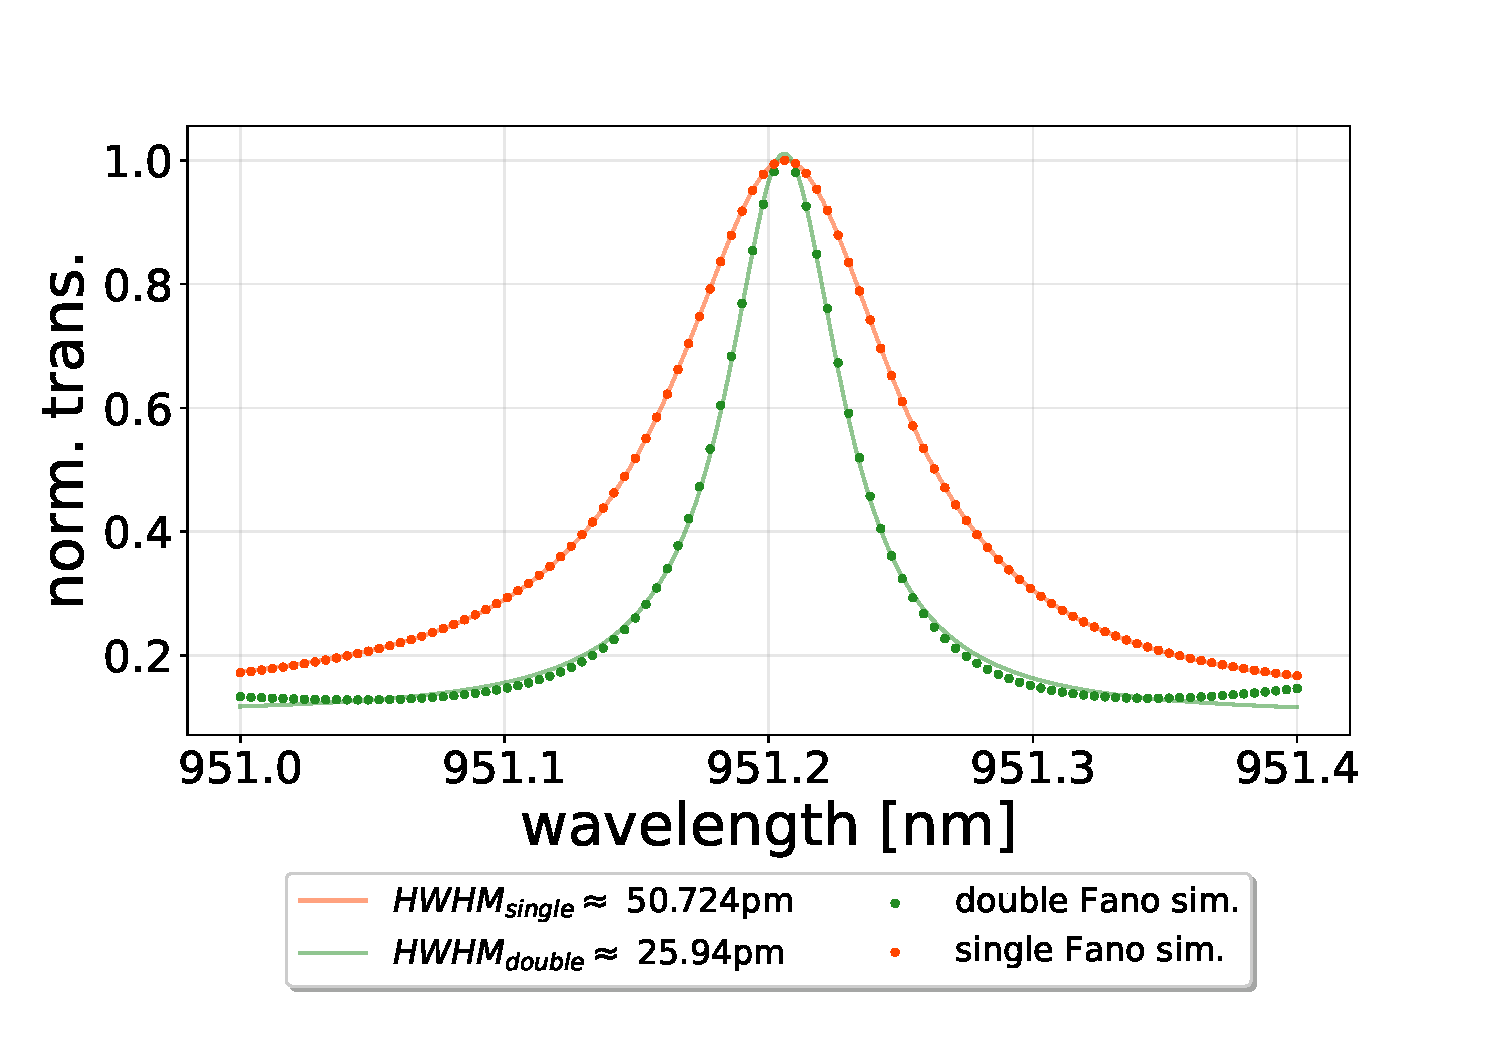
\includegraphics[width=\textwidth]{figures/sim_single_vs_double_10um.pdf}
        \caption{}
        \label{fig:single_vs_double_simulation_10um}
    \end{subfigure}
    \begin{subfigure}[b]{0.49\textwidth}
        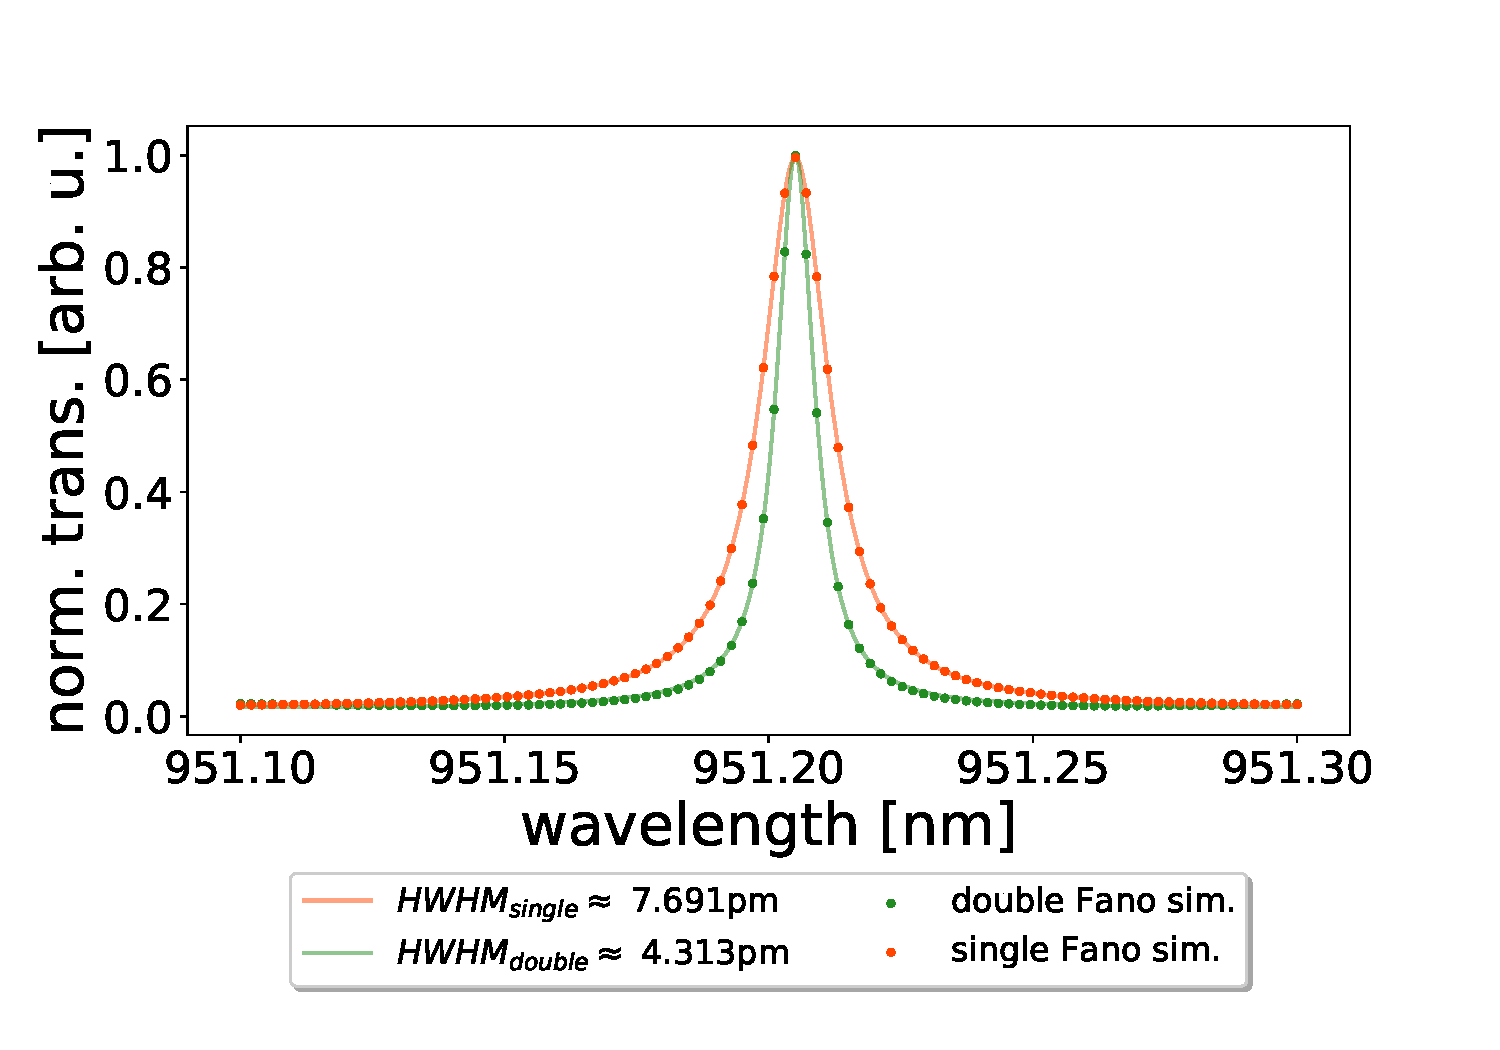
\includegraphics[width=\textwidth]{figures/sim_single_vs_double_30um.pdf}
        \caption{}
        \label{fig:single_vs_double_simulation_30um}
    \end{subfigure}
\end{figure}

\begin{figure}[h!]
    \centering
    \begin{subfigure}[b]{0.49\textwidth}
        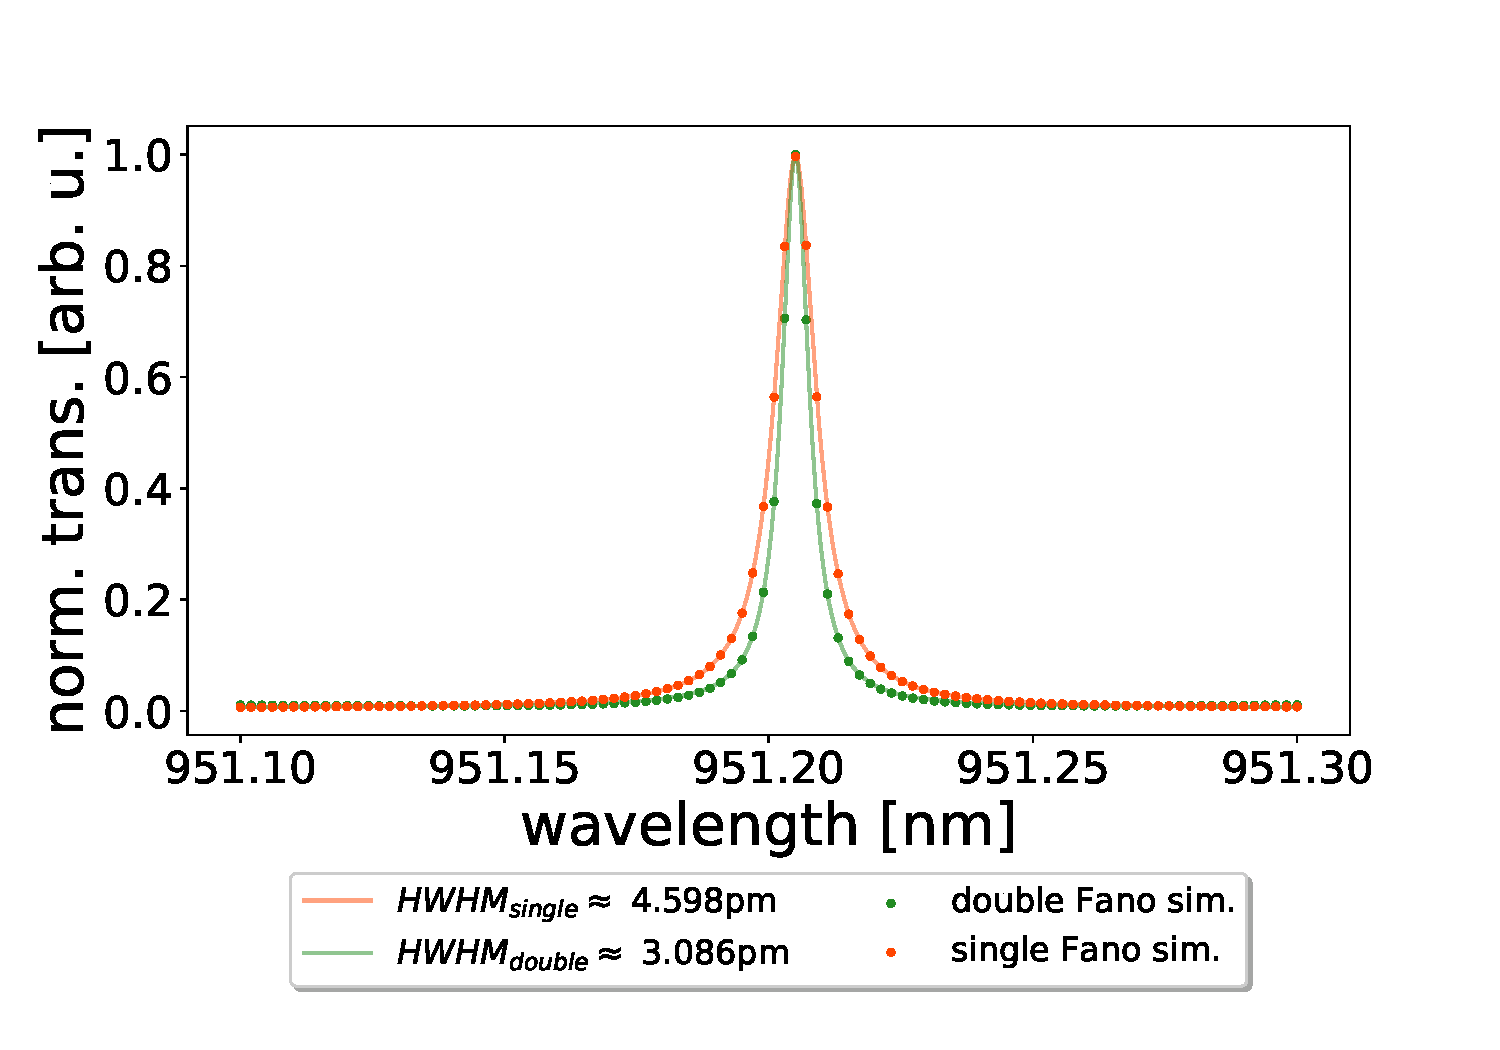
\includegraphics[width=\textwidth]{figures/sim_single_vs_double_90um.pdf}
        \caption{}
        \label{fig:single_vs_double_simulation_90um}
    \end{subfigure}
    \begin{subfigure}[b]{0.49\textwidth}
        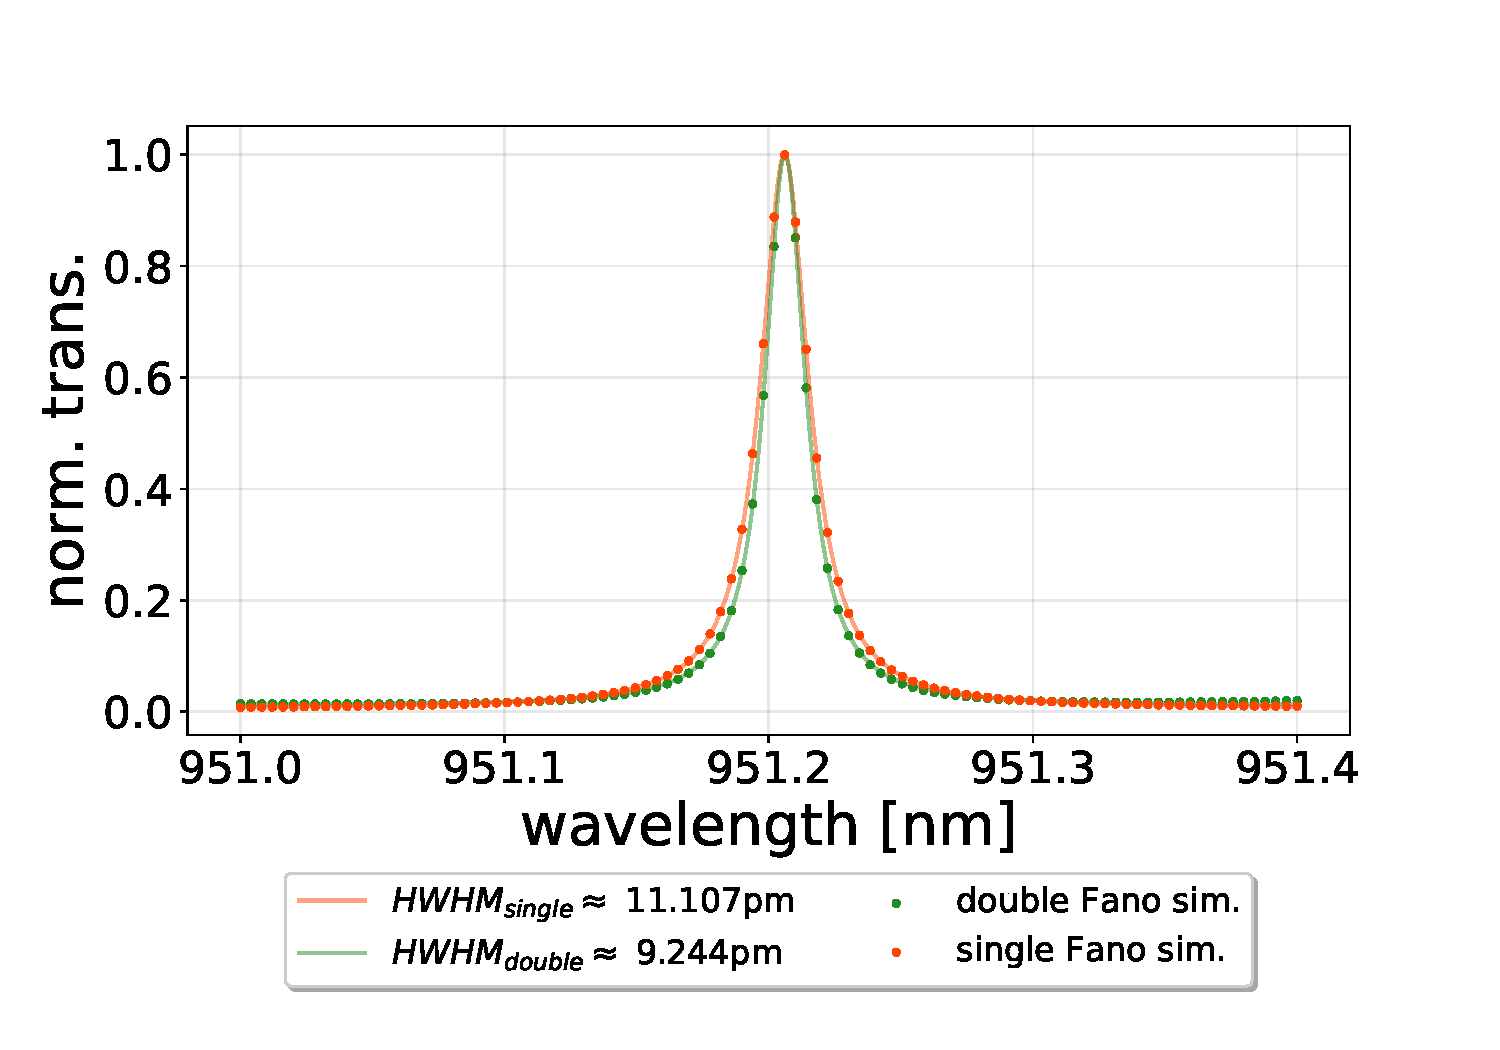
\includegraphics[width=\textwidth]{figures/sim_single_vs_double_270um.pdf}
        \caption{}
        \label{fig:single_vs_double_simulation_270um}
    \end{subfigure}
\end{figure}

\begin{figure}[h!]
    \centering
    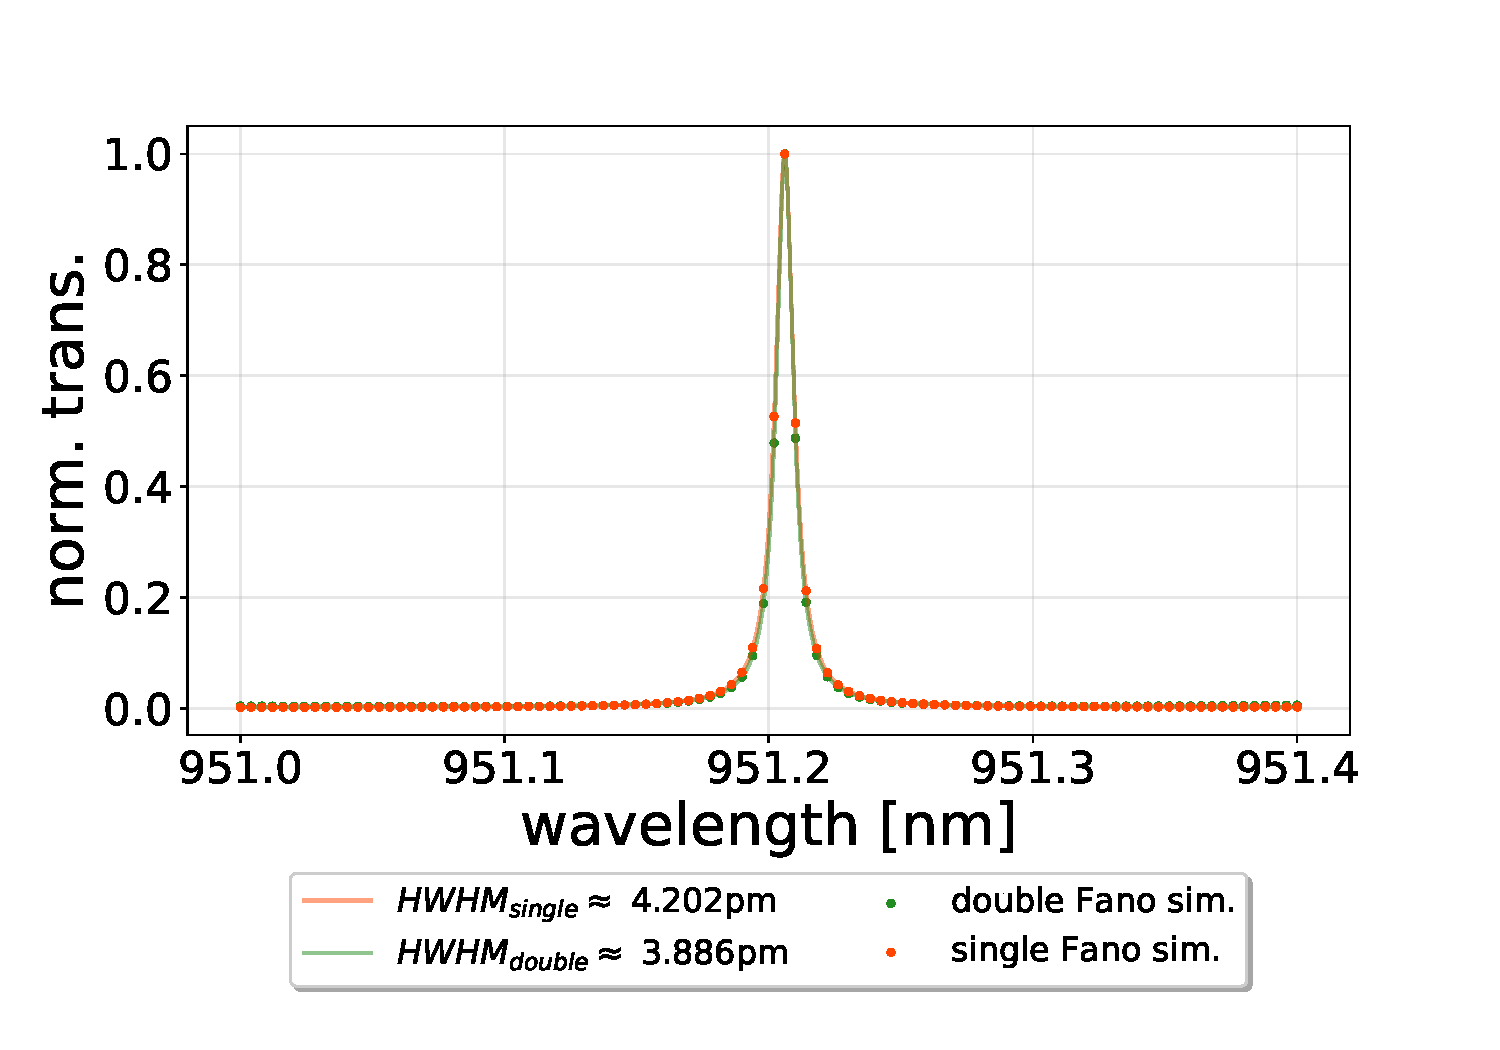
\includegraphics[width=0.49\textwidth]{figures/sim_single_vs_double_810um.pdf}
    \caption{}
    \label{fig:single_vs_double_simulation_810um}
\end{figure}

\subsection{Simulated double Fano cavity resonance transmission spectra for different values of the resonant loss term}

\begin{figure}[h!]
    \centering
    \begin{subfigure}[b]{0.49\textwidth}
        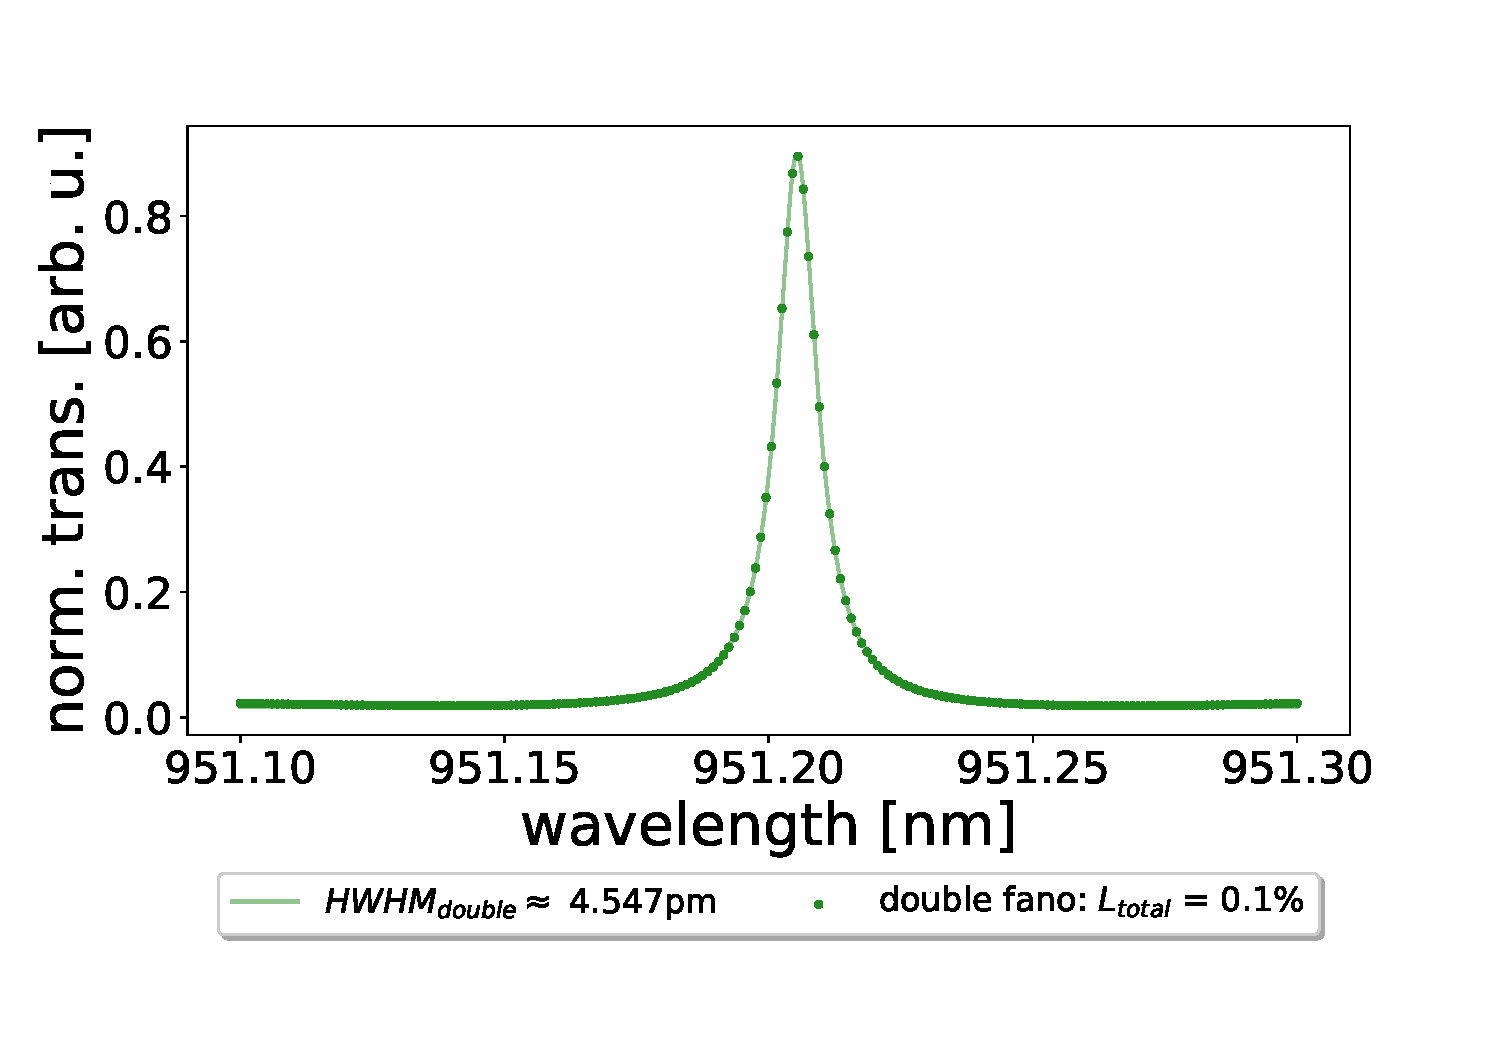
\includegraphics[width=\textwidth]{figures/double_01_percent_loss_30um.pdf}
        \caption{}
        \label{fig:0.1_percent_loss}
    \end{subfigure}
    \begin{subfigure}[b]{0.49\textwidth}
        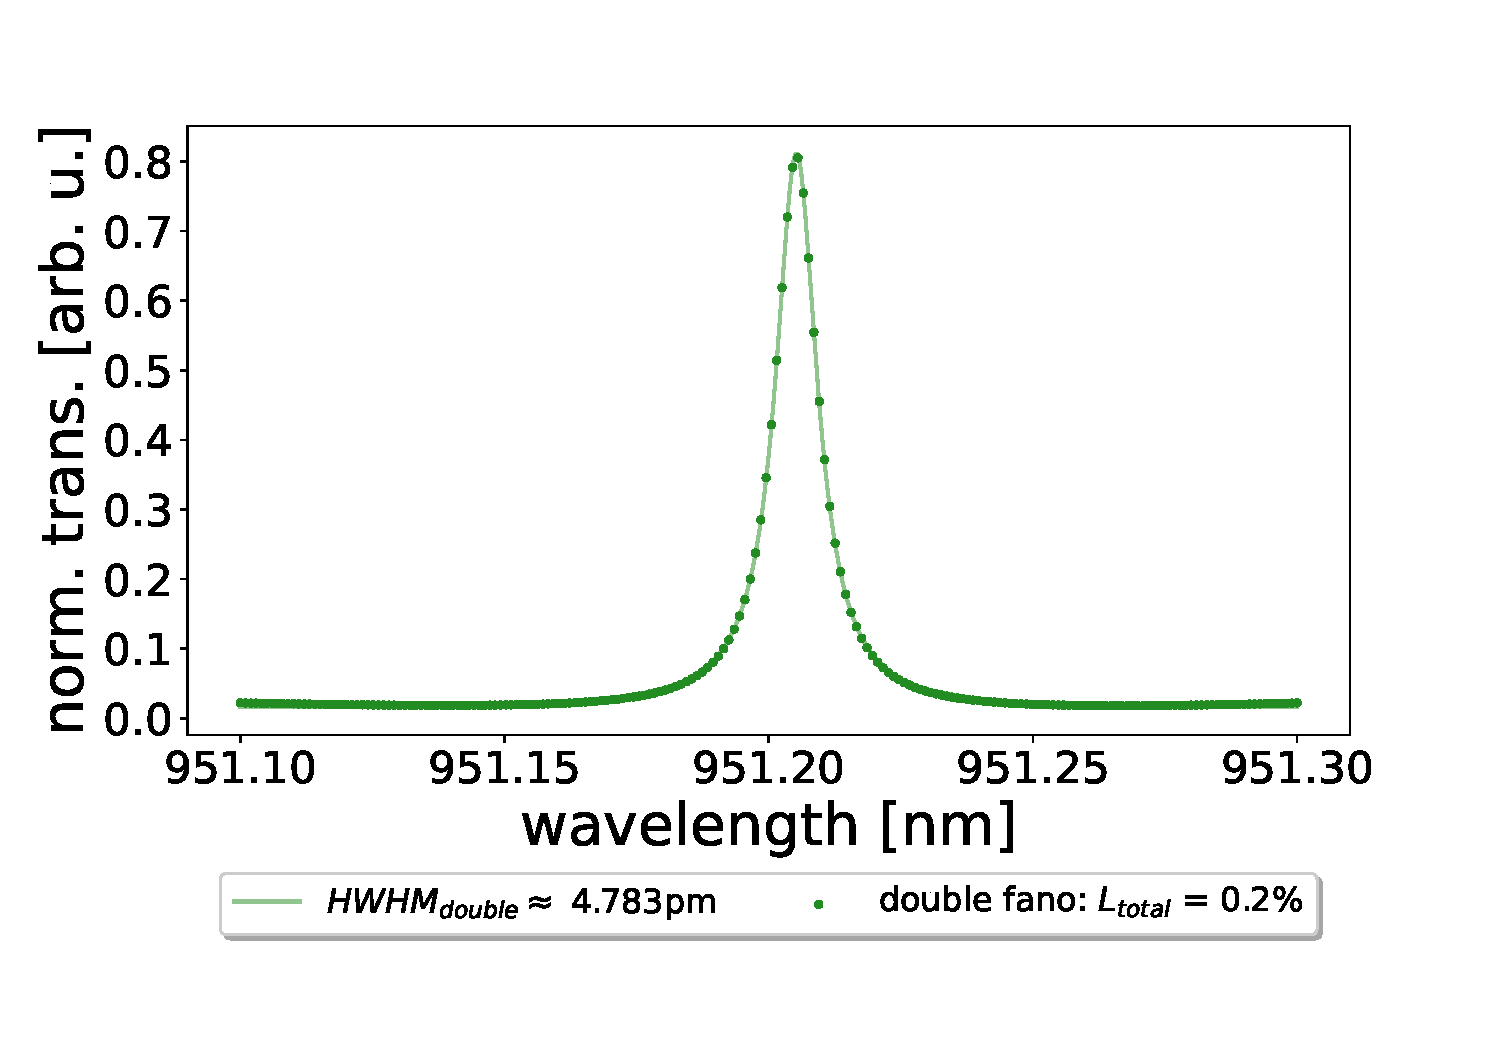
\includegraphics[width=\textwidth]{figures/double_02_percent_loss_30um.pdf}
        \caption{}
        \label{fig:0.2_percent_loss}
    \end{subfigure}
\end{figure}

\begin{figure}[h!]
    \centering
    \begin{subfigure}[b]{0.49\textwidth}
        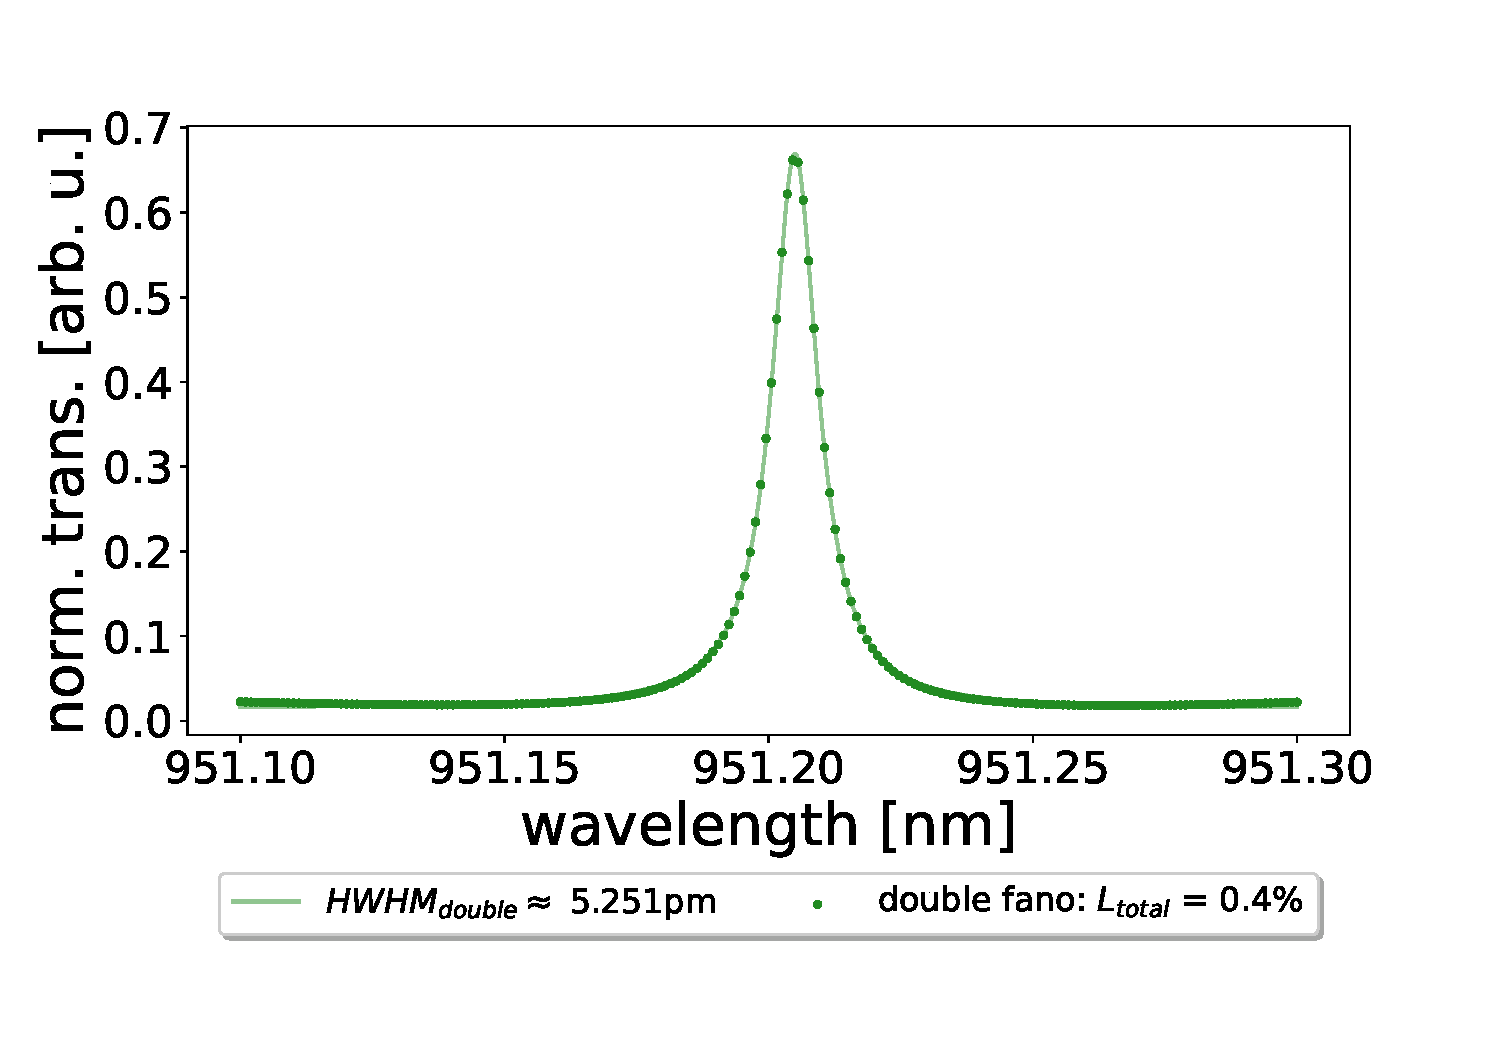
\includegraphics[width=\textwidth]{figures/double_04_percent_loss_30um.pdf}
        \caption{}
        \label{fig:0.4_percent_loss}
    \end{subfigure}
    \begin{subfigure}[b]{0.49\textwidth}
        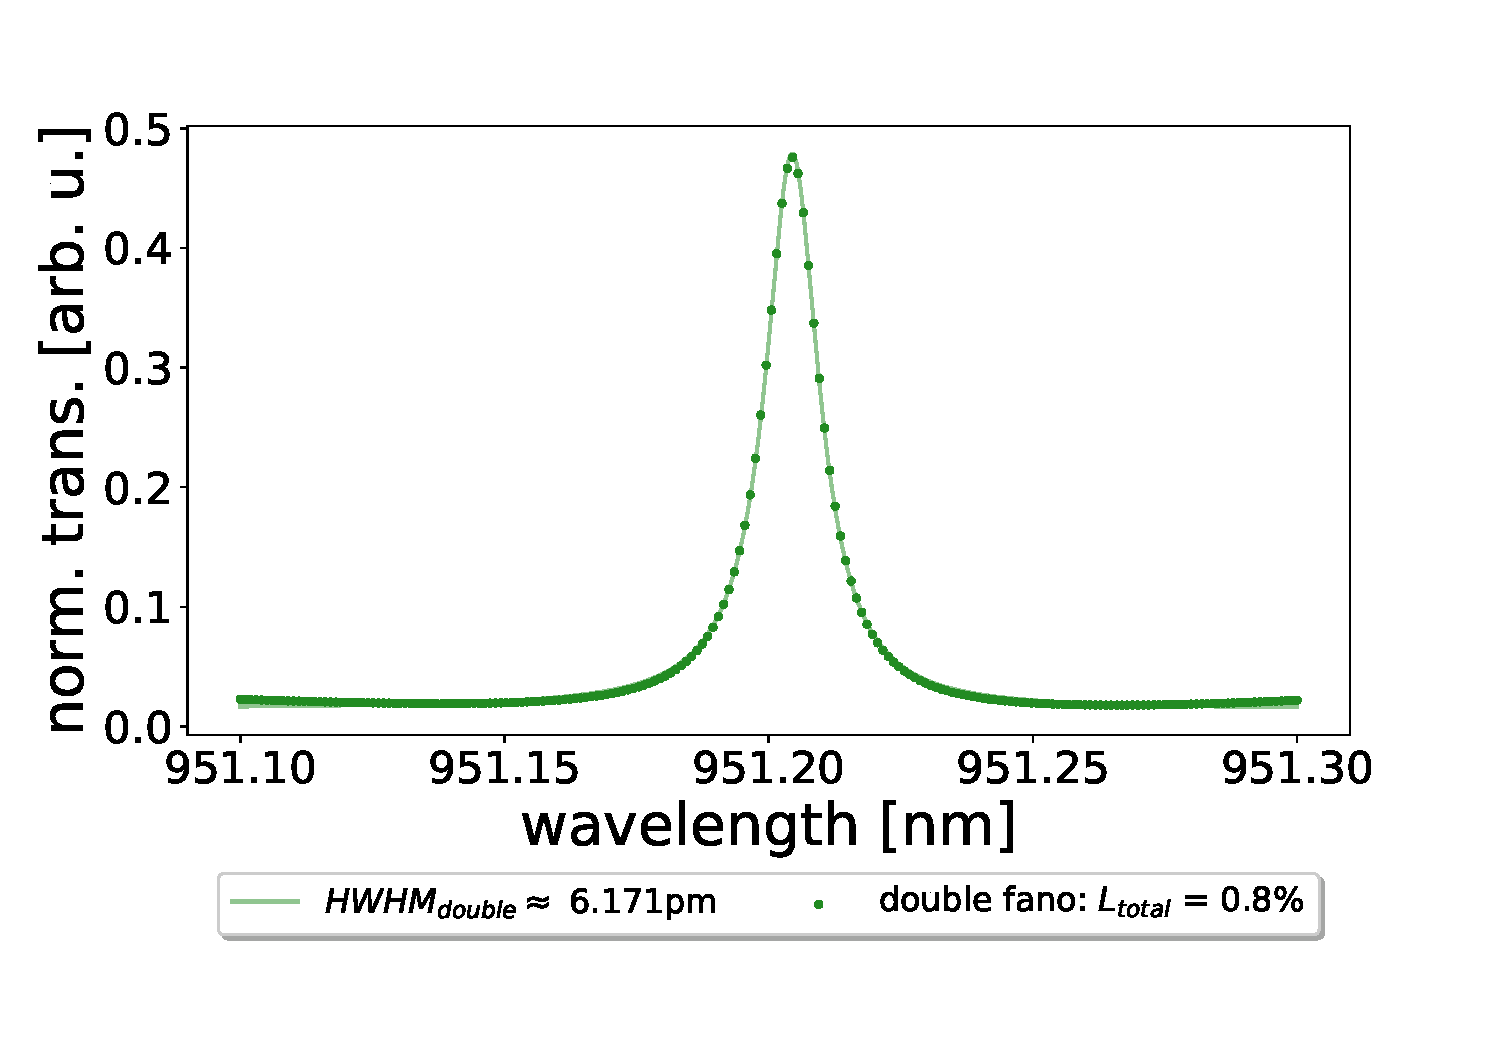
\includegraphics[width=\textwidth]{figures/double_08_percent_loss_30um.pdf}
        \caption{}
        \label{fig:0.8_percent_loss}
    \end{subfigure}
\end{figure}

\begin{figure}[h!]
    \centering
    \begin{subfigure}[b]{0.49\textwidth}
        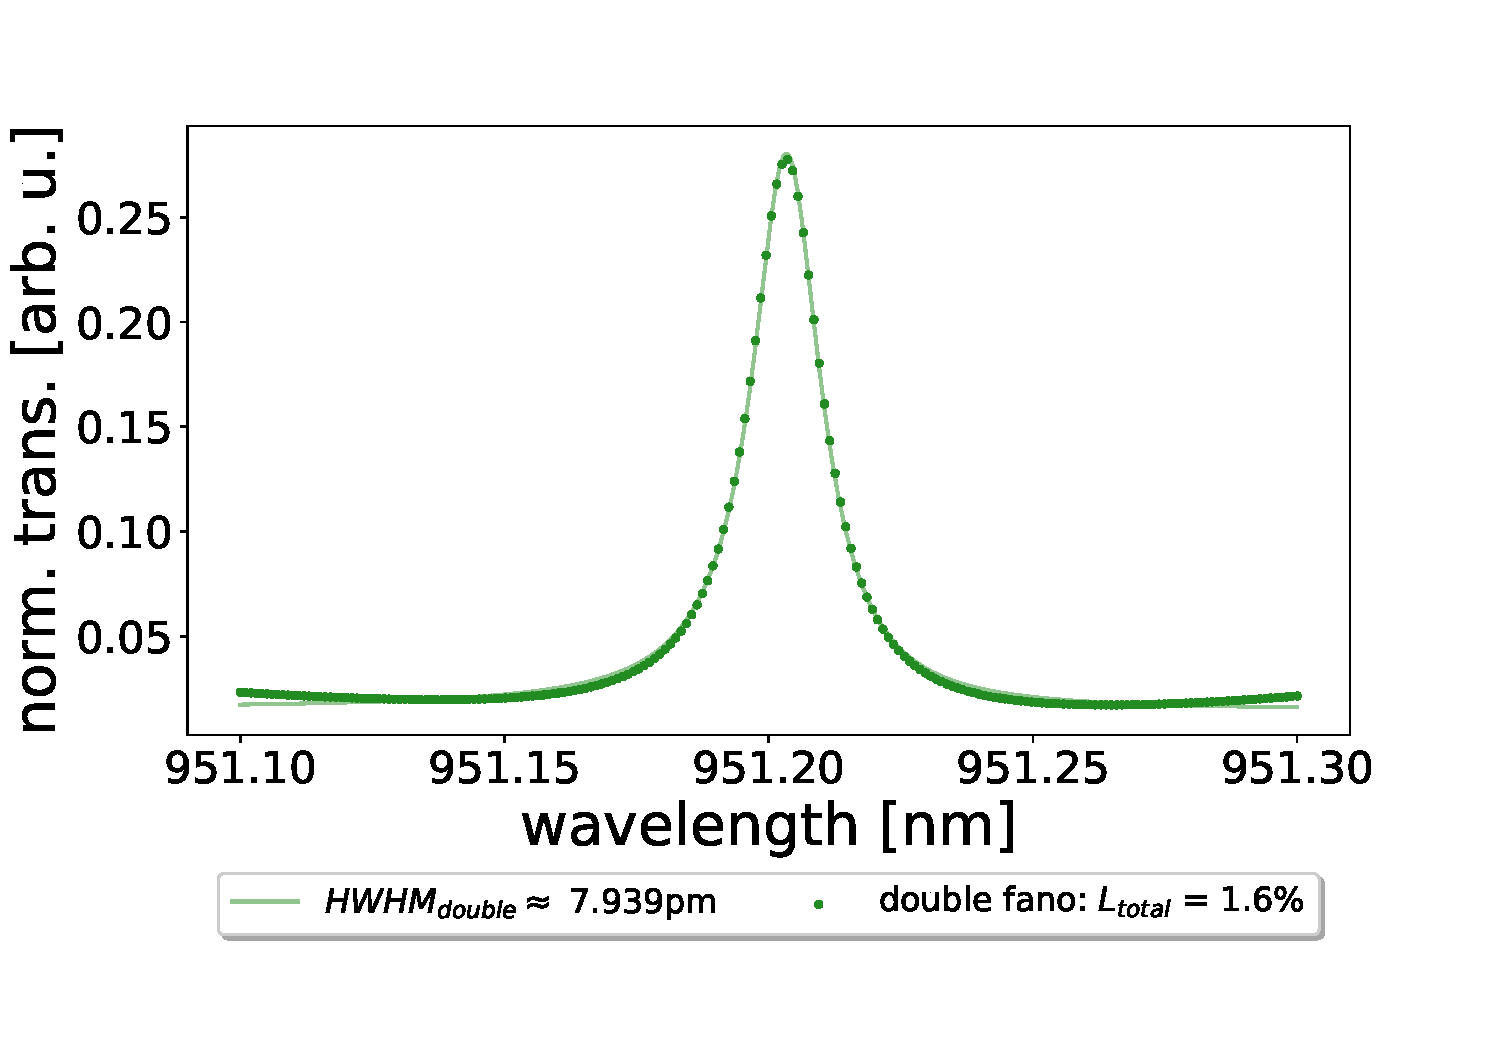
\includegraphics[width=\textwidth]{figures/double_16_percent_loss_30um.pdf}
        \caption{}
        \label{fig:1.6_percent_loss}
    \end{subfigure}
    \begin{subfigure}[b]{0.49\textwidth}
        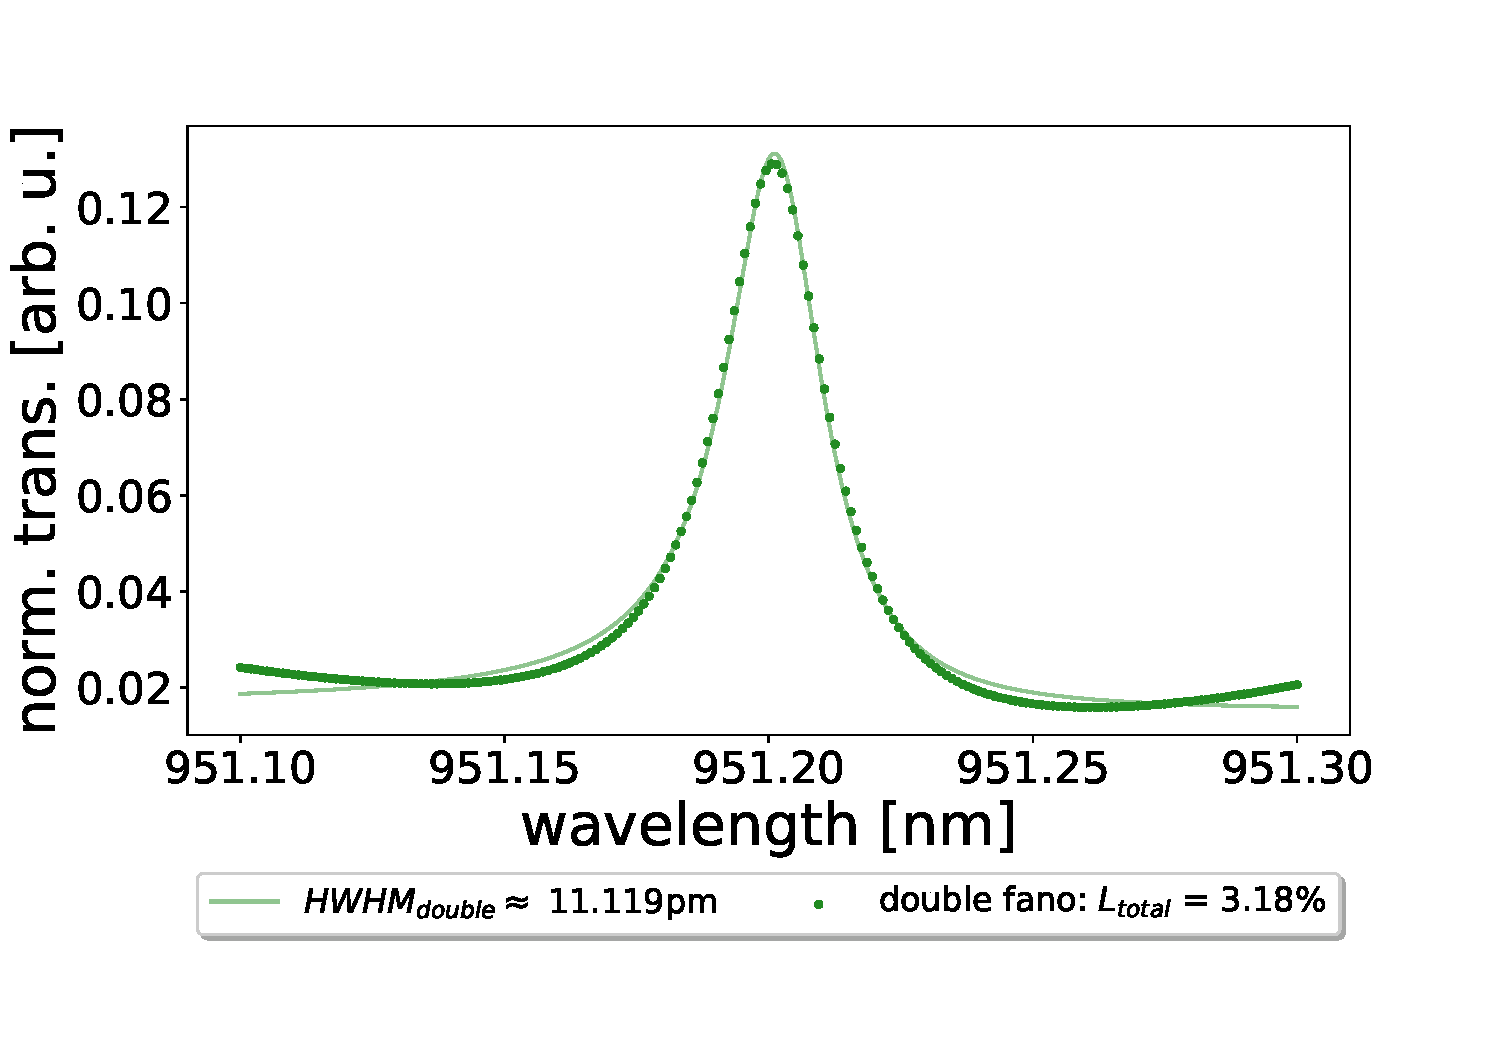
\includegraphics[width=\textwidth]{figures/double_32_percent_loss_30um.pdf}
        \caption{}
        \label{fig:3.2_percent_loss}
    \end{subfigure}
\end{figure}

\newpage
Things to add to appendix:
\begin{itemize}
    \item The derivation of equation \ref{eq:general_fano_model}
    \item The derivation of equation \ref{eq:analytical_linewidth}
    \item Same derivations for the double fano cavity.
\end{itemize}